%!TEX root = ./template-skripsi.tex
%-------------------------------------------------------------------------------
%                            BAB III
%               			PEMBAHASAN
%-------------------------------------------------------------------------------

\chapter{METODOLOGI PENELITIAN}

\section{Deskripsi Sistem}

\begin{figure}[H]
	\centering
	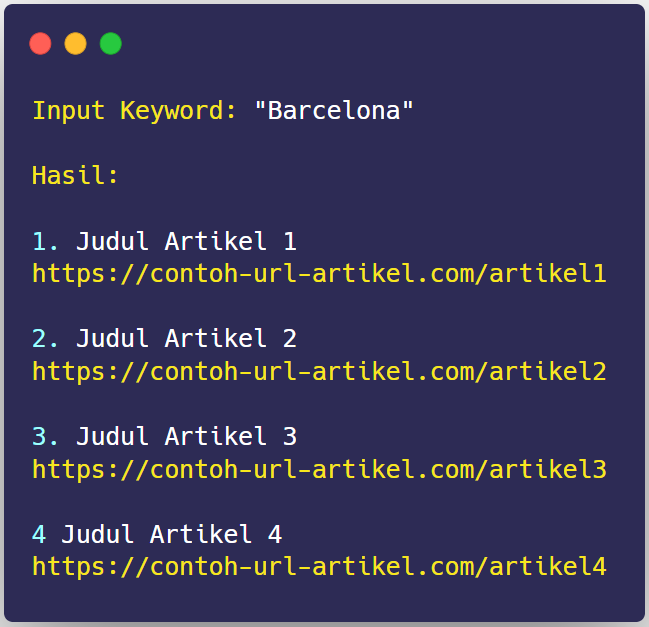
\includegraphics[keepaspectratio, width=8cm]{gambar/tampilan_sistem}
	\caption{\textit{Wireframe} Tampilan Sistem}
	\label{gambar:tampilan_sistem}
\end{figure}

Sistem yang akan dibuat pada penelitian ini adalah sistem \textit{search engine} yang berfungsi untuk pencarian \textit{website} berbasis \textit{terminal} yang akan menerima \textit{input} berupa \textit{keyword} dari pengguna dan sistem akan menampilkan hasil \textit{website} yang relevan sesuai dengan \textit{keyword} tersebut.

Pembuatan \textit{search engine} ini menggunakan beberapa algoritma dan metode sebagai pendukungnya, yaitu algoritma \textit{modified similarity based crawling} yang terdapat pada komponen \textit{crawler}, metode \textit{TF-IDF} untuk memberikan bobot pada dokumen berdasarkan \textit{keyword}, dan metode \textit{Google PageRank} untuk perangkingan \textit{website}. Selain itu, proses pengembangan sistem ini memakai metode pengembangan Scrum.

\begin{figure}[H]
	\centering
	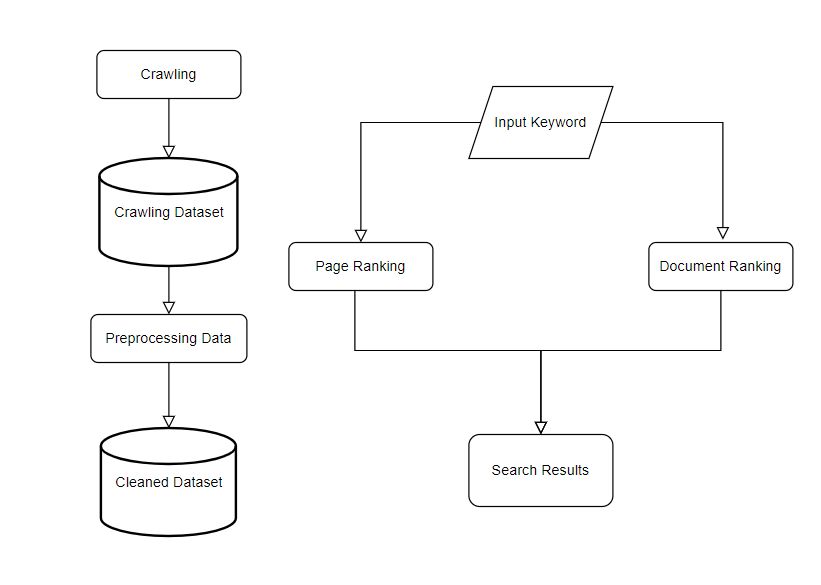
\includegraphics[keepaspectratio, width=13cm]{gambar/flowchart_sistem}
	\caption{\textit{Flowchart} Sistem}
	\label{gambar:flowchart_sistem}
\end{figure}

Proses dari sistem \textit{search engine} dimulai dengan mengumpulkan data ke dalam \textit{database} sebanyak-banyaknya menggunakan \textit{crawler}, lalu data tersebut akan diolah melalui \textit{preprocessing data} dan disimpan ke dalam \textit{database}. Setelah data sudah siap, maka sistem dimulai dengan meminta \textit{input} berupa \textit{keyword} dari pengguna lalu \textit{keyword} tersebut akan diproses melalui \textit{page ranking} dan \textit{document ranking}. Setelah itu hasil pencarian akan muncul sesuai dengan \textit{keyword} yang dimasukkan.

\section{Desain Penelitian}

Agar penelitian lebih terstruktur dan memudahkan penulis melakukan penelitian, maka dibutuhkan desain penelitian. Desain penelitian mencakup tahapan-tahapan yang dilakukan penulis dalam pembuatan sistem dengan menggunakan metode Scrum. Tahapan tersebut dapat dilihat pada gambar \ref{gambar:desain_penelitian}.

\begin{figure}[H]
	\centering
	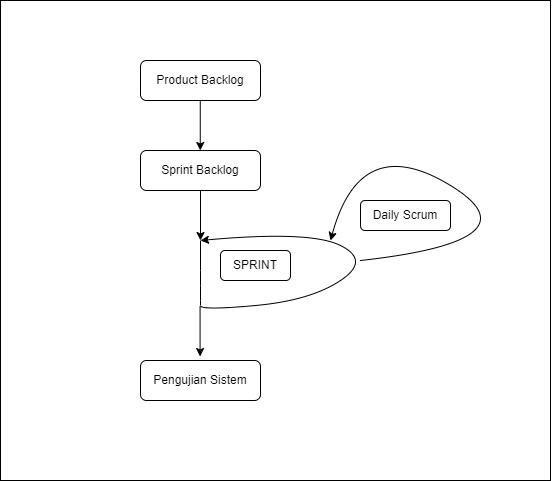
\includegraphics[keepaspectratio, width=13cm]{gambar/desain_penelitian}
	\caption{Desain Penelitian}
	\label{gambar:desain_penelitian}
\end{figure}

Tahap pertama yang dilakukan pada penelitian ini adalah mendefinisikan \textit{product backlog} dari sistem yang akan dibuat, lalu membuat jadwal pengerjaan atau \textit{sprint backlog}. Setelah itu, \textit{sprint} dimulai dengan diselingi \textit{daily scrum} untuk melaporkan \textit{progress} dan menentukan \textit{task} selanjutnya. Setelah sistem selesai dikerjakan di dalam \textit{sprint}, maka dilakukan pengujian sistem.

\section{Alat dan Bahan Penelitian}

Dalam penelitian ini, beberapa alat berupa perangkat keras yang digunakan untuk menunjang pembuatan sistem adalah sebagai berikut:

\begin{enumerate}

\item{Laptop yang mempunyai CPU Intel i7-6700hq dan RAM 20GB}
\item{LCD Monitor dengan resolusi 1920 x 1080 \textit{pixel}}
\item{Koneksi berbasis \textit{Wi-Fi}}

\end{enumerate}

Perangkat keras di atas sudah memenuhi persyaratan untuk menjalankan aplikasi \textit{Python} sebagai \textit{server} maupun sebagai \textit{interpreter} dan dapat menjalankan \textit{server} untuk \textit{database} \textit{MySQL}. Selain perangkat keras, perangkat lunak yang dipakai untuk membuat sistem ini adalah sebagai berikut:

\begin{enumerate}

\item{Windows 10 64-bit Operating System}
\item{Visual Studio Code sebagai \textit{code editor}}
\item{XAMPP untuk menjalankan \textit{MySQL database}}
\item{Python 3 untuk menjalankan program Python}

\end{enumerate}

\section{Perancangan Sistem}

Perancangan sistem pada penelitian ini sesuai dengan komponen yang ada di dalam metode Scrum. Komponen-komponen tersebut terdiri dari \textit{product backlog}, \textit{sprint backlog}, \textit{sprint}, \textit{daily scrum}, dan \textit{pengujian sistem}. Berikut merupakan rincian dari perancangan sistem sesuai dengan komponen Scrum.

\subsection{\textit{Product Backlog}}

Berikut merupakan tabel \textit{product backlog} sistem \textit{search engine} yang telah dibuat berdasarkan diskusi dengan \textit{Scrum Master}. Transkrip percakapan dengan \textit{Scrum Master} terdapat pada \textbf{Lampiran A}. Setiap \textit{item} dari \textit{product backlog} ini akan diimplementasikan pada \textit{sprint} dari awal hingga selesai.

\begin{table}[H]
	\caption{\textit{Product Backlog}}
	\label{product_backlog}
	\begin{tabular}{@{} |p{0.5cm}|p{7cm}|p{1.5cm}|p{2cm}|p{2cm}| @{}}
		\hline
		\textbf{No} & \textbf{\textit{Story}} & \textbf{\textit{Sprint}} & \textbf{\textit{Status}} & \textbf{\textit{Priority}} \\
		\hline
		1 & Mengubah struktur project dari program \textit{crawler} menjadi modular & 1 & Completed & Penting \\
		\hline
		2 & Konfigurasi program \textit{crawler} sebagai \textit{background service} di sistem operasi & 2 & & Penting \\
		\hline
		3 & Perancangan struktur \textit{package}, \textit{class}, dan fungsi program \textit{TF IDF} & 3 & & Penting \\
		\hline
		4 & Perancangan struktur \textit{package}, \textit{class}, dan fungsi program \textit{Page Rank} & 4 & & Penting \\
		\hline
		5 & Konfigurasi program \textit{page rank} sebagai \textit{background service} di sistem operasi & 5 & & Penting \\
		\hline
		6 & Merancang \textit{REST API} untuk fungsi utama \textit{TF IDF} & 6 & & Penting \\
		\hline
		7 & Perancangan struktur \textit{project} arsitektur \textit{search engine} & 7 & & Penting \\
		\hline
		8 & Perancangan struktur kode untuk modul pengindeks \textit{Generalized Suffix Tree} & 8 & & Penting \\
		\hline
	\end{tabular}
\end{table}

Berdasarkan tabel \ref{product_backlog} di atas, \textit{Product Backlog} pada penelitian ini terdiri dari 4 komponen, yaitu \textit{story}, \textit{sprint}, \textit{status}, dan \textit{priority}. \textit{Story} menggambarkan pekerjaan besar yang nantinya akan dipecah lagi menjadi \textit{task-task} yang kecil di dalam \textit{Sprint}. Komponen \textit{sprint} pada tabel ini menandakan \textit{sprint} berapa \textit{story} tersebut akan dilaksanakan. Komponen \textit{status} menjelaskan apakah \textit{story} tersebut sudah selesai atau belum.  Sedangkan komponen \textit{priority} menjelaskan skala prioritas dari \textit{story} tersebut.

\subsection{\textit{Sprint Backlog}}

\textit{Sprint backlog} adalah daftar pekerjaan yang perlu dikerjakan ataupun yang sudah dikerjakan pada \textit{sprint}. Di dalam \textit{sprint backlog}, berbagai \textit{task} kecil dibuat berdasarkan \textit{story} yang terdapat pada \textit{product backlog}. Berikut merupakan rincian dari \textit{sprint backlog} yang pertama.

\begin{enumerate}

	\item{\textit{Sprint-1}}
	
	\textit{Sprint-1} dilakukan sepekan pada tanggal 16 April 2022 sampai dengan 22 April 2022. \textit{Story} pertama pada \textit{product backlog} dipecah menjadi beberapa \textit{task} sebagai berikut.
	
	\begin{table}[H]
	\caption{\textit{Sprint 1 Backlog}}
	\label{sprint1_backlog}
	\begin{tabular}{@{} |p{0.5cm}|p{5cm}|p{5cm}|p{2cm}| @{}}
		\hline
		\textbf{No} & \textbf{\textit{Story}} & \textbf{\textit{Task}} & \textbf{\textit{Status}} \\
		\hline
		1 & \multirow{13}{5cm}{Mengubah struktur kode dari program \textit{crawler} menjadi modular} & Membuat rancangan class diagram & Completed\\
		\cline{1-1}\cline{3-4}
		2 & & Membuat rancangan entity relationship diagram untuk database & Completed\\
		\cline{1-1}\cline{3-4}
		3 & & Mengubah struktur kode crawler sesuai dengan rancangan class diagram & Completed\\
		\cline{1-1}\cline{3-4}
		4 & & Implementasi threading untuk menjalankan lebih dari satu proses dalam satu waktu & Completed\\
		\cline{1-1}\cline{3-4}
		5 & & Testing program versi terbaru & Completed\\
		\hline
	\end{tabular}
	\end{table}
	
\end{enumerate}

\subsection{\textit{Daily Scrum}, \textit{Sprint Review}, dan \textit{Sprint Retrospective}}

Dikarenakan sumber daya dan waktu yang terbatas, aktivitas \textit{daily scrum} akan digantikan dengan cara mencatat hal-hal penting dan hambatan yang terjadi setiap hari sebagai \textit{note} di \textit{Github Projects}.

\textit{Sprint review}, dan \textit{sprint retrospective} dilakukan pada awal pekan yaitu di hari Selasa melalui \textit{voice call}. Pada awal pekan ini akan dilakukan evaluasi mengenai perkembangan sistem maupun hambatan yang terjadi selama pengerjaan di setiap \textit{sprint}.

\subsection{\textit{Sprint 1 Report}}

Setelah merencanakan \textit{sprint backlog}, pekerjaan pada \textit{sprint} ini harus mengikuti rencana kerja yang ditentukan oleh \textit{sprint backlog}. Tujuan dari \textit{sprint-1} ini adalah mengubah struktur kode program \textit{crawler} sebelumnya menjadi modular. Untuk manajemen \textit{task} dan \textit{progress},  penulis menggunakan \textit{GitHub Projects} seperti pada gambar \ref{gambar:sprint1_projects}.
	
\begin{figure}[H]
	\centering
	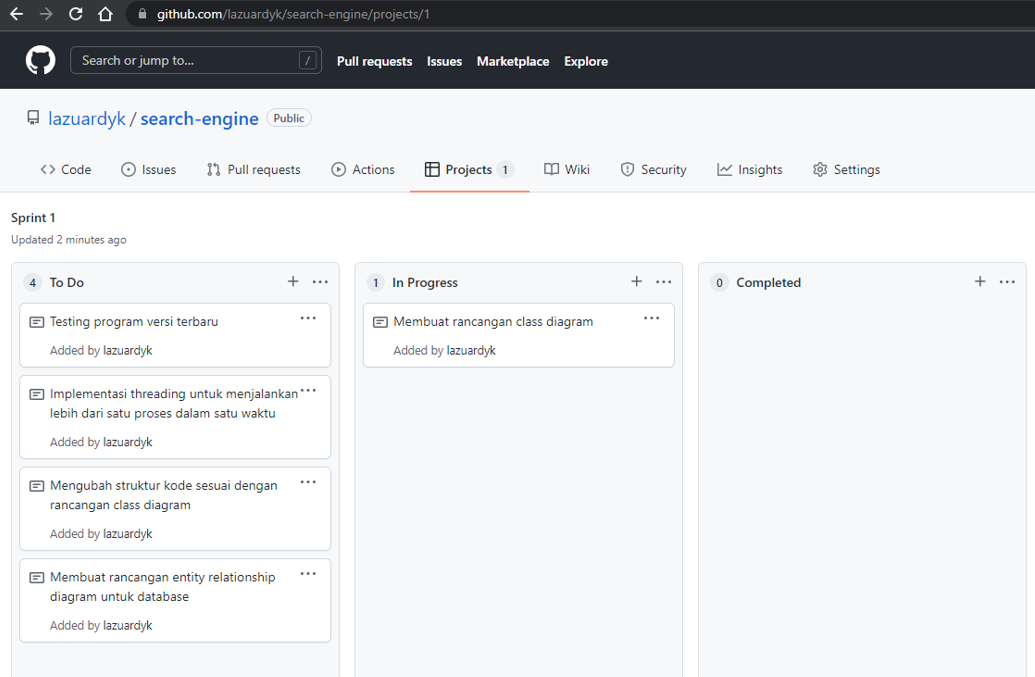
\includegraphics[keepaspectratio, width=14cm]{gambar/sprint1_projects}
	\caption{\textit{Github Projects Sprint-1}}
	\label{gambar:sprint1_projects}
\end{figure}
	
Terdapat 3 kolom pada \textit{project} yang dibuat, yaitu \textit{to do}, \textit{in progress}, dan \textit{completed}. Setiap \textit{task} yang perlu dikerjakan akan ditulis dan dimasukkan ke dalam kolom \textit{to do}, \textit{task} yang sedang dikerjakan akan dipindahkan ke kolom \textit{in progress}, dan jika task sudah selesai akan dipindahkan ke kolom \textit{completed}. Berikut merupakan hasil dari pengerjaan yang dilakukan selama \textit{sprint 1}.

\begin{enumerate}
	
	\item{\textit{Entity Relationship Diagram Database}}
	
	\textit{Entity Relationship Diagram (ERD)} pada \textit{sprint-1} ini menggambarkan masing-masing entitas dan relasi antar entitas pada \textit{database} untuk \textit{crawler}.
	
	\begin{figure}[H]
	\centering
	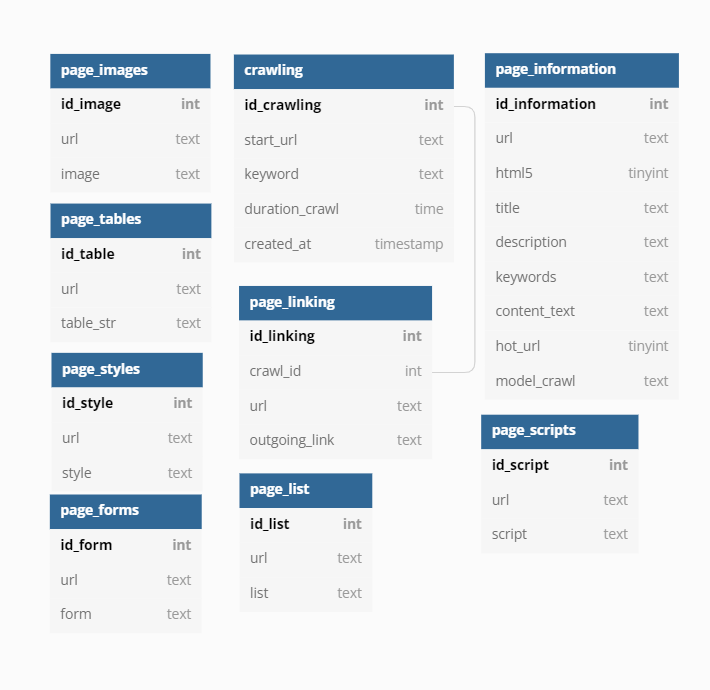
\includegraphics[keepaspectratio, width=13cm]{gambar/sprint1_erd}
	\caption{\textit{Entity Relationship Diagram Sprint-1}}
	\label{gambar:sprint1_erd}
	\end{figure}
	
	Tabel-tabel yang dibutuhkan untuk menyimpan data pada \textit{crawler} yaitu tabel \textit{crawling}, \textit{page\_linking}, \textit{page\_information}, \textit{page\_images}, \textit{page\_tables}, \textit{page\_styles}, \textit{page\_forms}, \textit{page\_list}, dan \textit{page\_scripts}.
	
	\item{\textit{Class Diagram}}
	
	\textit{Class diagram} pada gambar \ref{gambar:sprint1_class_diagram} menggambarkan kelas-kelas dalam sistem yang dipakai \textit{crawler}. Rancangan tersebut merupakan rancangan \textit{class diagram} dari program \textit{crawler} yang modular.
	
	\begin{figure}[H]
	\centering
	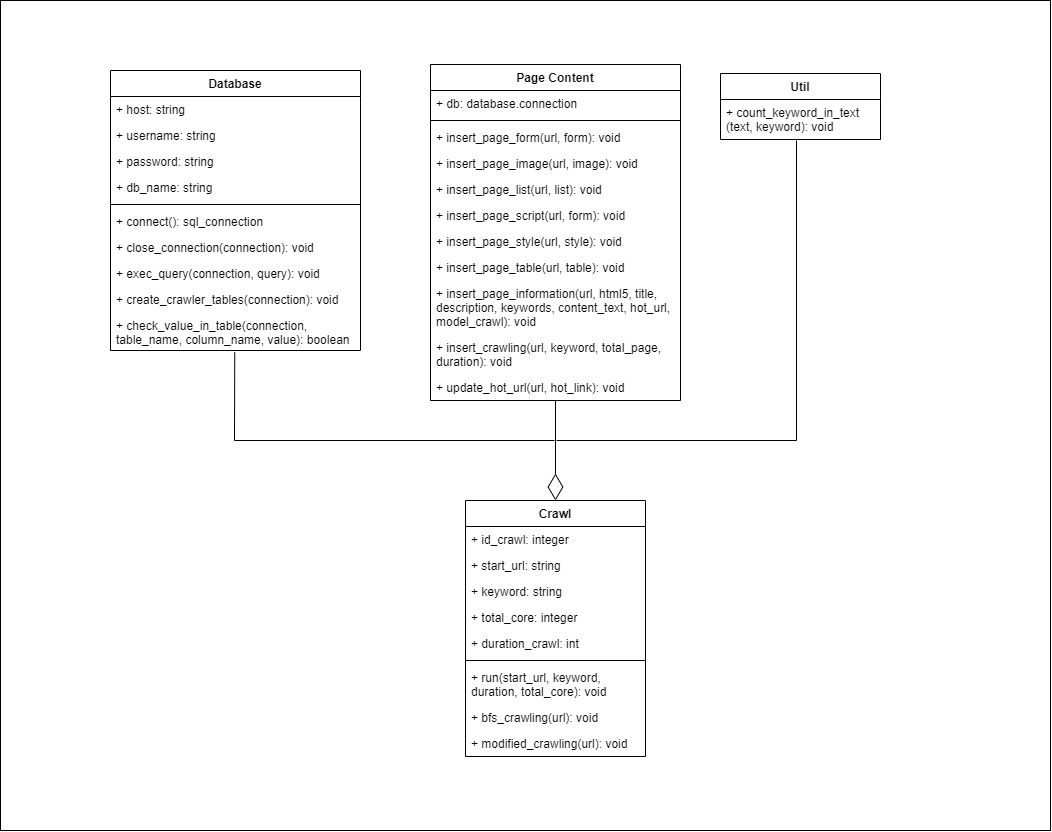
\includegraphics[keepaspectratio, width=15cm]{gambar/sprint1_class_diagram}
	\caption{\textit{Class Diagram Sprint-1}}
	\label{gambar:sprint1_class_diagram}
	\end{figure}
	
	Pada rancangan\textit{ class diagram crawler} ini, terdapat 4 kelas yang akan dibuat, yaitu kelas \textit{database} untuk koneksi dan pembuatan \textit{table} pada \textit{database}, kelas \textit{page content} yang berisi fungsi-fungsi untuk menyimpan konten dari halaman \textit{website}, kelas \textit{util} yang terdapat fungsi-fungsi pendukung, dan kelas \textit{crawl} sebagai kelas utama untuk menjalankan \textit{crawler}.
	
	\item{\textit{Source code}}
	
	\textit{Source code} dari \textit{sprint-1} terdapat di \textit{Github Repository}, yang dapat diakses pada link https://github.com/lazuardyk/search-engine/tree/sprint-1
	
	\item{Pengujian Sistem \textit{Crawler}}
	
	Pengujian sistem dilakukan dengan menjalankan program \textit{crawler} yang dilakukan penelitian sebelumnya dan versi yang terbaru melalui \textit{terminal command prompt} dan menargetkan situs https://www.indosport.com/ dengan \textit{keyword} berupa "barcelona". Kedua program tersebut dijalankan selama 2 jam dan pada versi crawler terbaru menggunakan 3 \textit{threads} karena menerapkan konsep \textit{multithreading}.
	
	\begin{figure}[H]
	\centering
	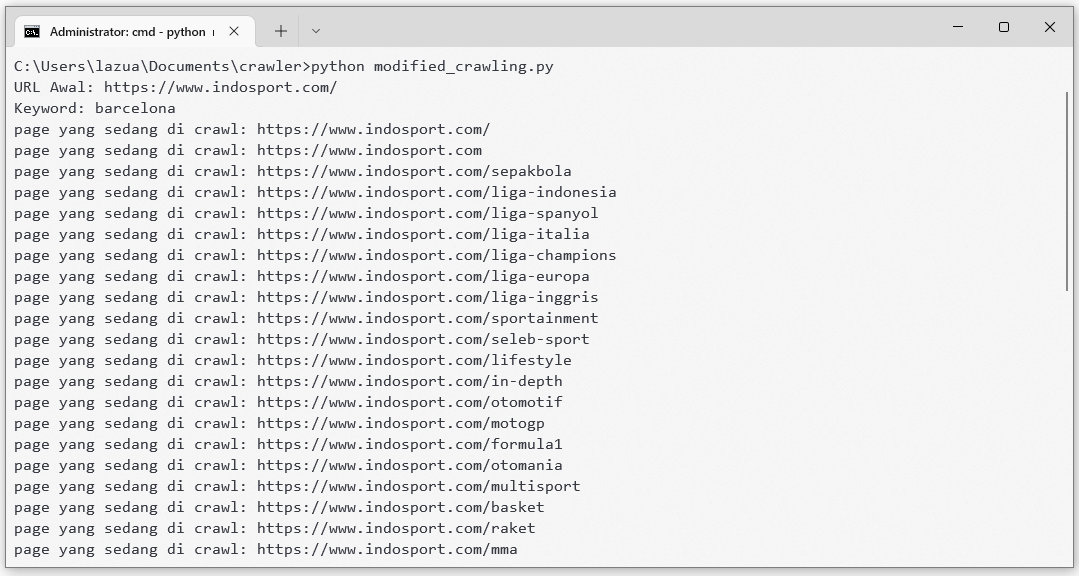
\includegraphics[keepaspectratio, width=13cm]{gambar/sprint1_testing1_old}
	\caption{Pengujian \textit{crawler} penelitian sebelumnya}
	\label{gambar:sprint1_testing1_old}
	\end{figure}
	
	\begin{figure}[H]
	\centering
	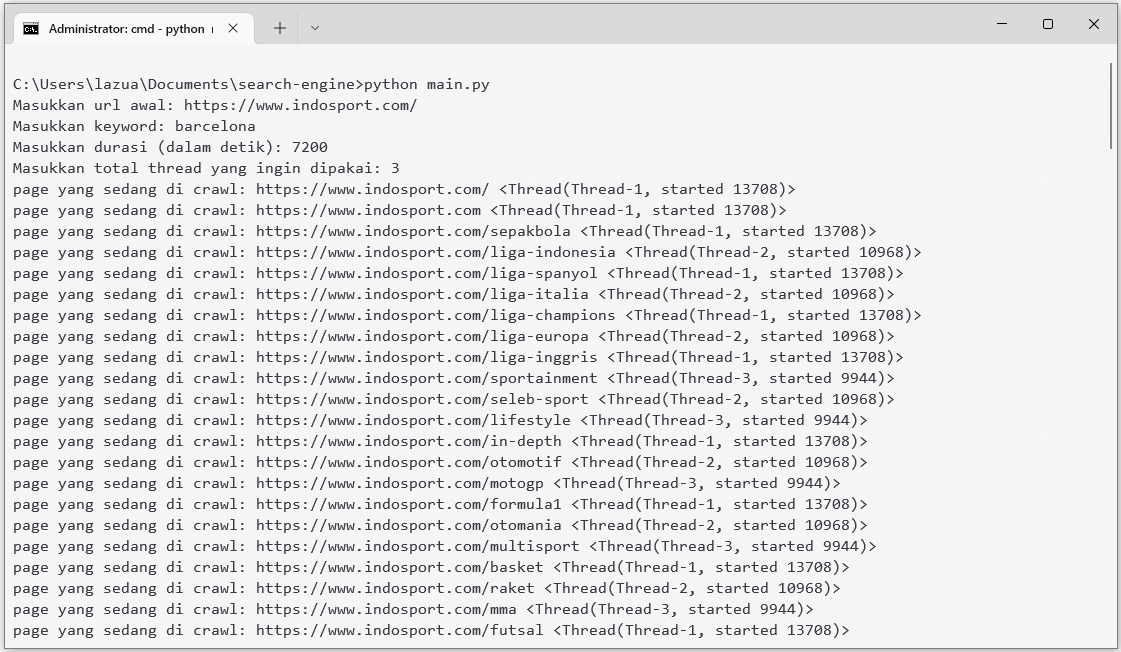
\includegraphics[keepaspectratio, width=13cm]{gambar/sprint1_testing1}
	\caption{Pengujian \textit{crawler} versi terbaru}
	\label{gambar:sprint1_testing1}
	\end{figure}
	
	Gambar \ref{gambar:sprint1_testing1_old} dan gambar \ref{gambar:sprint1_testing1} merupakan tampilan \textit{crawler} versi lama dan terbaru yang berjalan setelah dimasukkan \textit{input} dari \textit{user}. Hasil dari kedua \textit{crawler} yang telah selesai dijalankan ini terdapat pada gambar \ref{gambar:sprint1_testing2_old} dan gambar \ref{gambar:sprint1_testing2}.
	
	\begin{figure}[H]
	\centering
	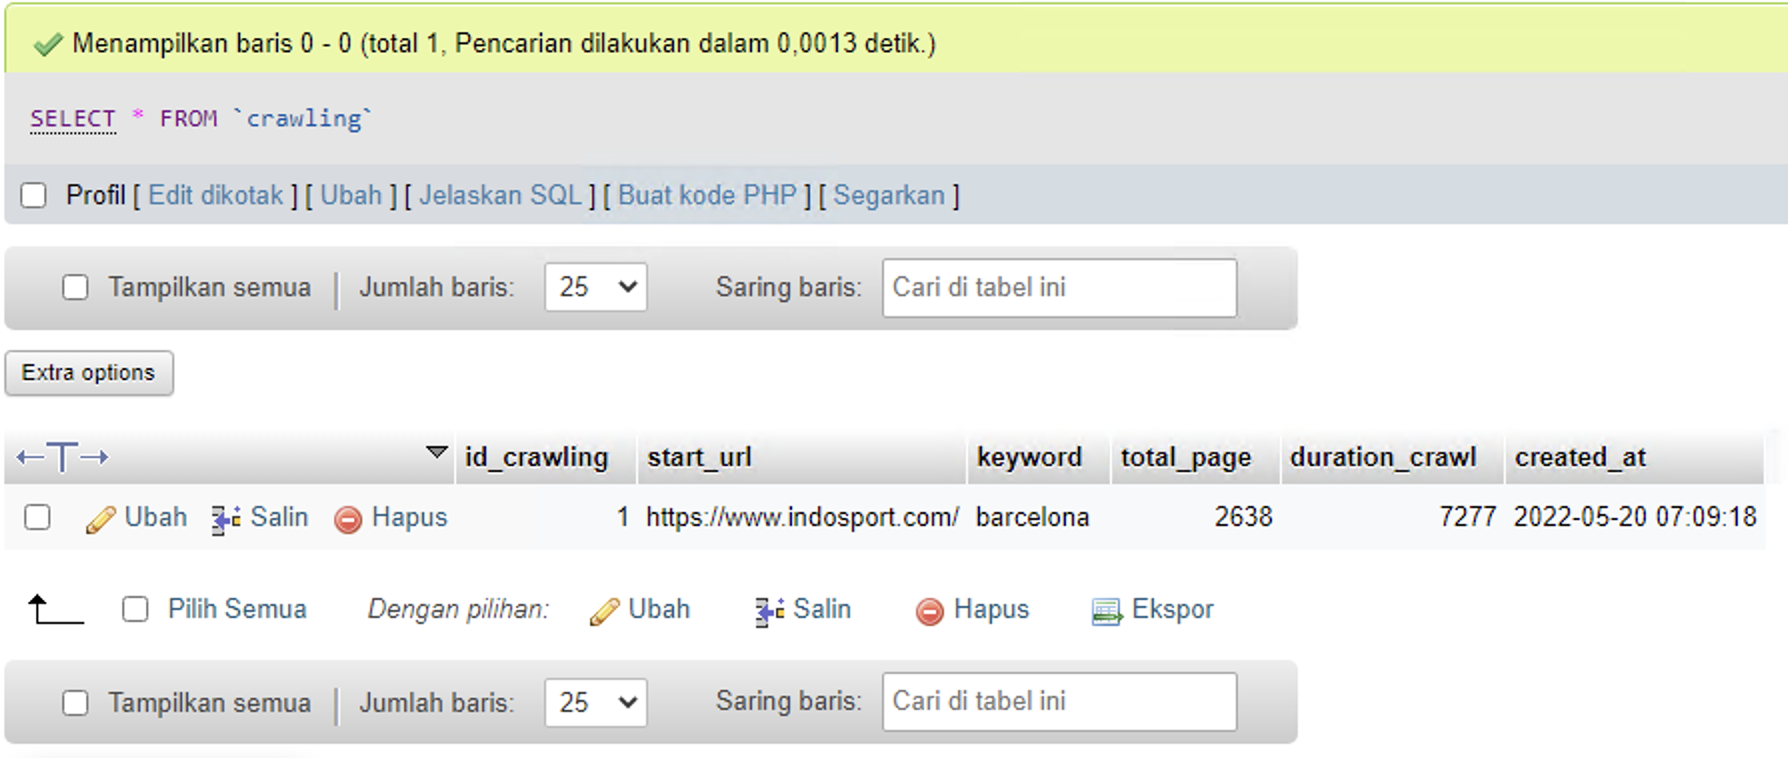
\includegraphics[keepaspectratio, width=13cm]{gambar/sprint1_testing2_old}
	\caption{Hasil pengujian \textit{crawler} penelitian sebelumnya}
	\label{gambar:sprint1_testing2_old}
	\end{figure}
	
	\begin{figure}[H]
	\centering
	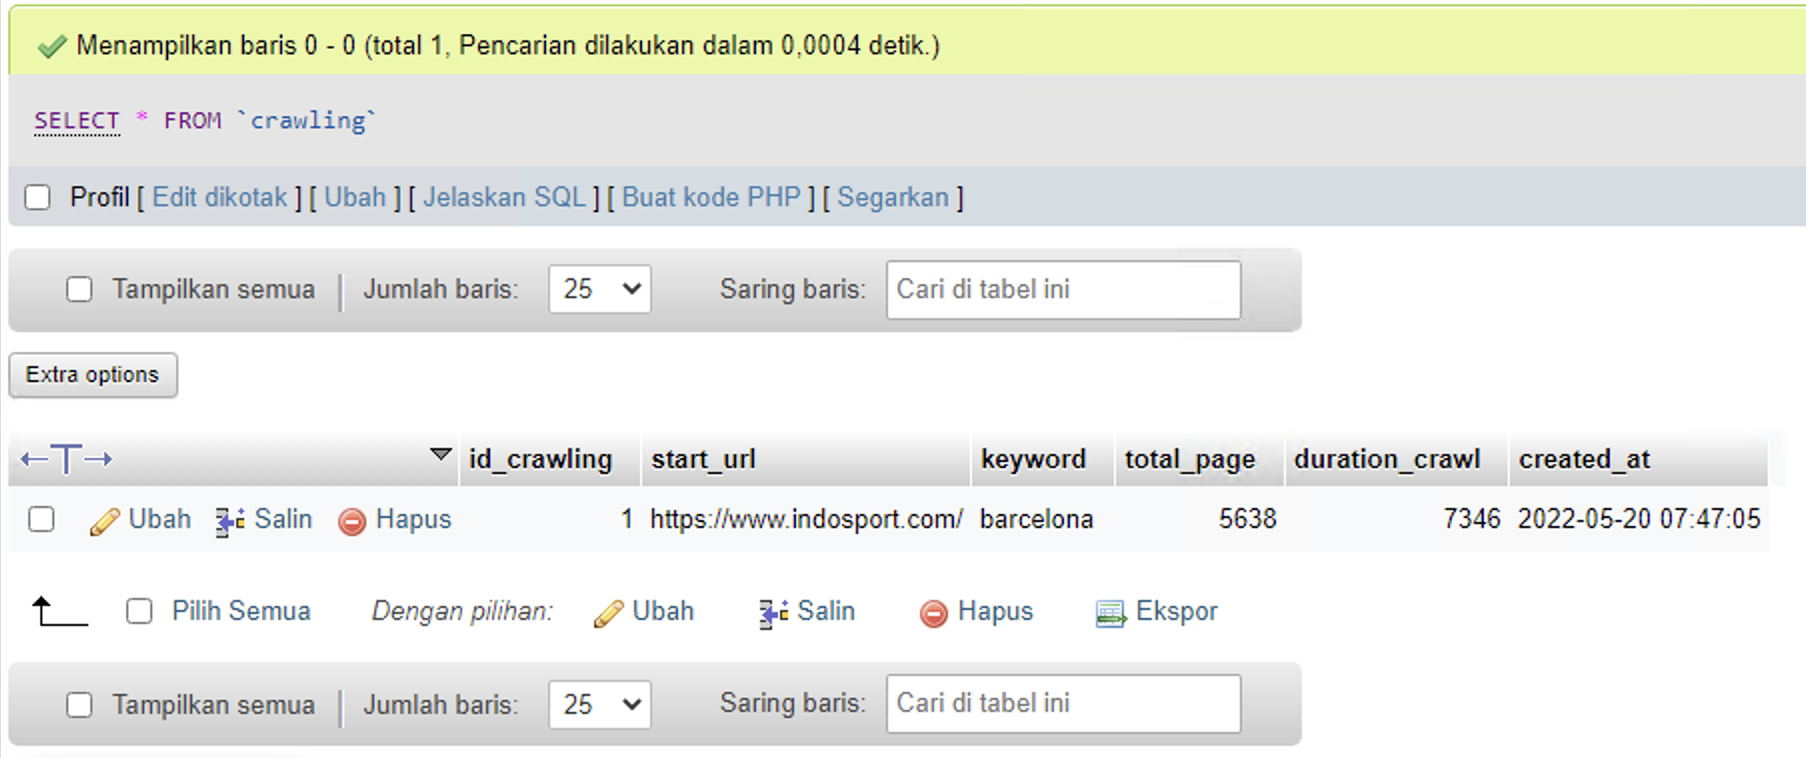
\includegraphics[keepaspectratio, width=13cm]{gambar/sprint1_testing2}
	\caption{Hasil pengujian \textit{crawler} versi terbaru}
	\label{gambar:sprint1_testing2}
	\end{figure}
	
	Untuk situs awal https://www.indosport.com/ hasil yang didapat pada \textit{crawler} penelitian sebelumnya adalah 2638 halaman dengan durasi 7277 detik, sedangkan pada \textit{crawler} versi terbaru adalah 5638 halaman dengan durasi 7346 detik. Dengan demikian, waktu yang dibutuhkan untuk \textit{crawling} satu halaman adalah 2,7 detik pada \textit{crawler} versi lama dan 1,3 detik pada \textit{crawler} terbaru yang saat ini dikembangkan.
	
	\begin{figure}[H]
	\centering
	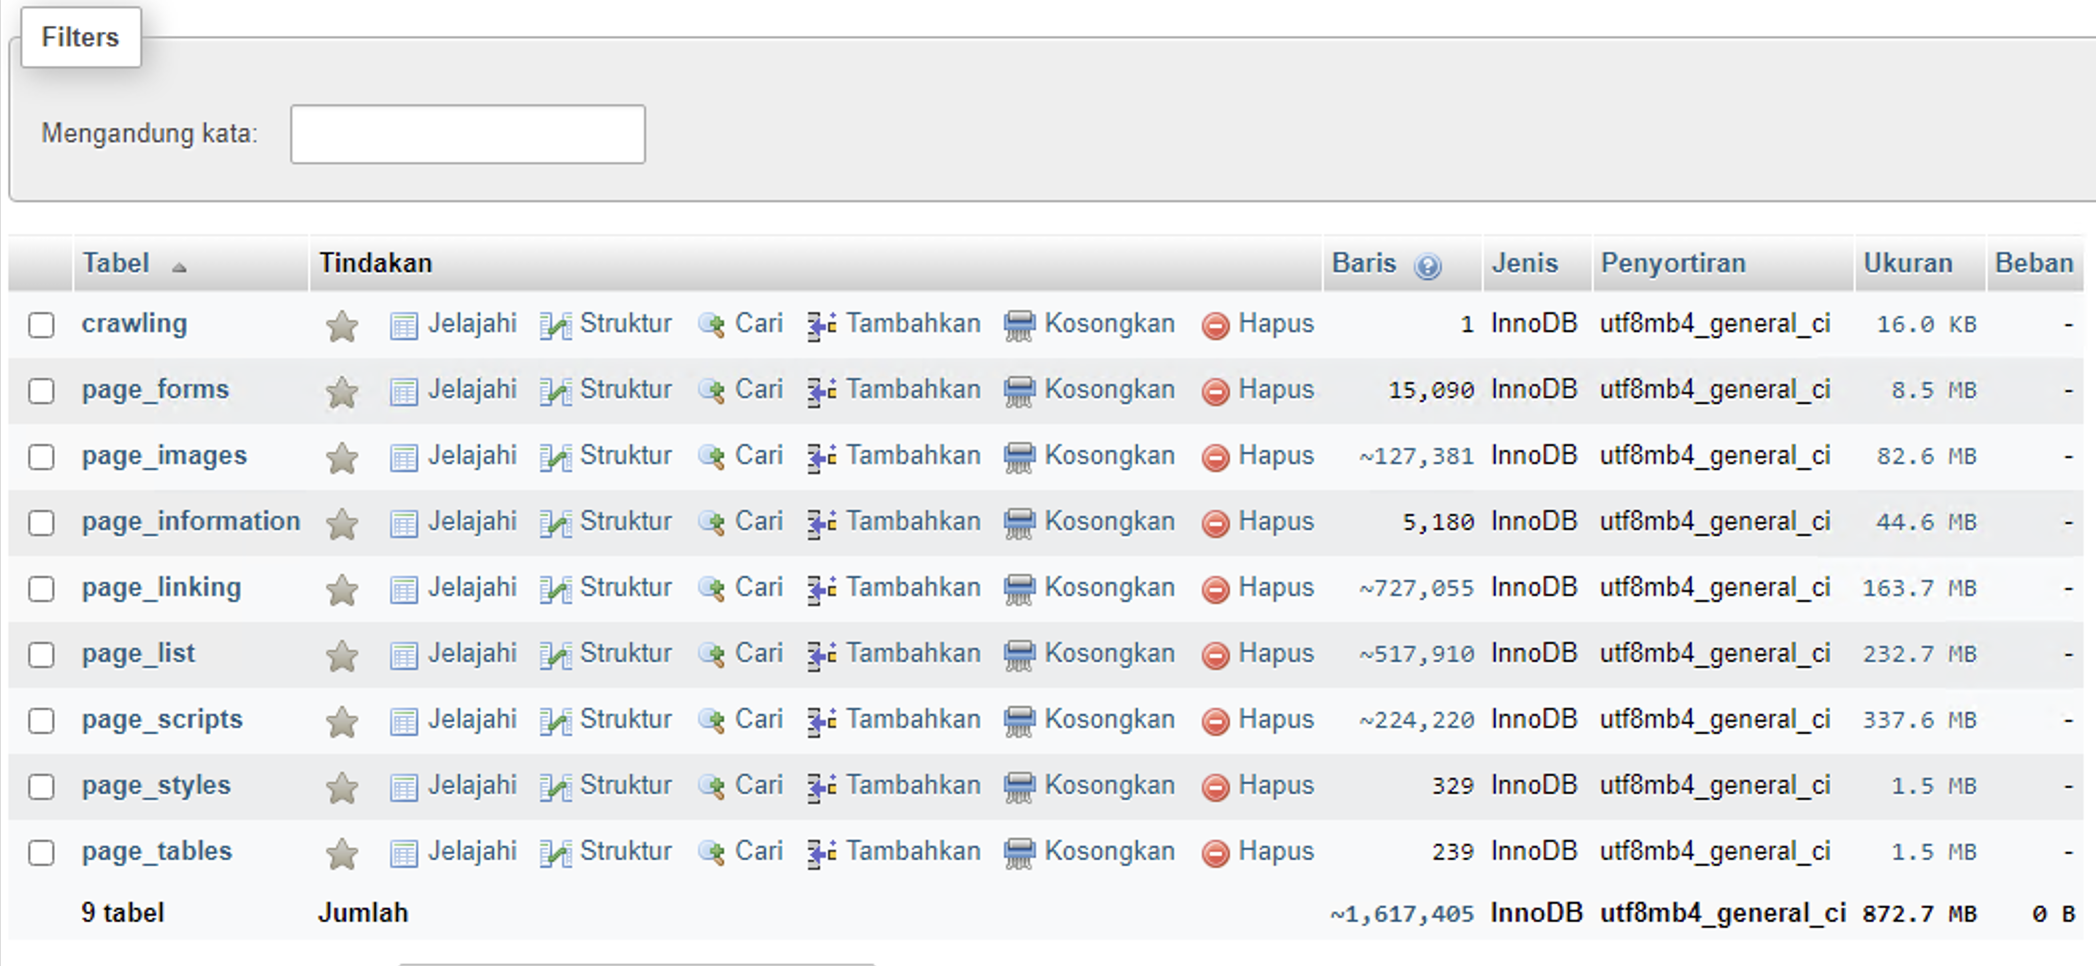
\includegraphics[keepaspectratio, width=13cm]{gambar/sprint1_testing3}
	\caption{Hasil pengujian \textit{crawler} terbaru 2}
	\label{gambar:sprint1_testing3}
	\end{figure}
	
	Konten \textit{website} yang diperoleh dari proses pengujian \textit{crawling} pada \textit{crawler} versi terbaru untuk setiap tabelnya adalah 15.090 baris pada \textit{page\_forms}, 127.381 baris pada \textit{page\_images}, 5.180 baris pada \textit{page\_information}, 727.055 baris pada \textit{page\_linking}, 517.910 baris pada \textit{page\_list}, 224.220 baris pada page\_scripts, 329 baris pada \textit{page\_styles}, dan 239 baris pada \textit{page\_tables}.

\end{enumerate}


%\subsection{\textit{Daily Scrum}}

%Pada akhir pekan di akhir setiap \textit{sprint}, akan diadakan \textit{voice call} untuk membahas perkembangan dan hambatan pada setiap \textit{sprint}.